\section{The Path to Victory}

Suppose we have an undirected graph $G$ that is a \textit{path}: namely, its nodes can be written as $v_1, v_2, \ldots v_n$ with an edge between $v_i$ and $v_j$ if and only if $i$ and $j$ are consecutive numbers. Each node $v_i$ has a positive weight $w_i$. For example, in the following path, the weights are shown as numbers drawn inside the nodes:

\begin{figure*}[tbh!]
	\centering
	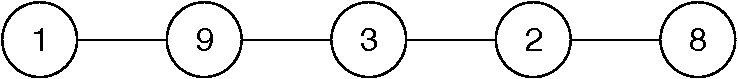
\includegraphics[width=0.6\textwidth]{path.pdf}
\end{figure*}

In this problem, we want to find the \textit{maximum independent set}. An independent set is a subset of nodes such that no two of them share and edge, and the maximum independent set is the independent set with largest total weight. For example, in the graph above, the largest-weight independent set is $v_2$ and $v_5$, with total weight 17.

Assume you're given an $n$-dimensional array $V$, where $V[i]$ contains the weight of the node $v_i$ (note that we are assuming 1-based indexing).

\begin{questions}
	\question[3] Give a recurrence $M(i)$ (for $0 \le i \le n$) that defines the weight of the maximum independent set of the first $i$ nodes in $G$.

	\ifsolutions\begin{soln}
	Let \(G = (V, E)\) be a graph such that it is a tournament. Let \(i \in V\) be the node such that it has maximum out-degree.

	We aim to prove that \(\forall j \neq i \in V\) either \(i\) beat \(j\) or \(i\) beat \(k \in V\) who beat \(j\) for any size \(|V| = n \in \mathbb{N}\).

	Base case: \(|V| = 2\). Then if \(i\) has max out-degree then \(E = \{(i, j)\}\). Thus, the claim holds.

	Assume the claim holds for \(|V| = n\), with \(n \in \mathbb{N}\).

	Consider a tournament with \(|V| = n + 1\) nodes. Denote the player who has maximum out-degree by \(i\).

	Then remove \(j \neq i\) from this graph, so that we have \(n\) nodes, denote \(V' = V\setminus \{j\}\), with \(i\) beat \(j\).

	Either \(i\) has the maximum out-degree in this graph or not. We consider each case.

	\begin{itemize}
		\item \text{Case \(i\) has maximum out-degree in \(V'\)}. Then, by assumption for each node other node \(j' \in V'\), either \(i\) beat \(j'\) or \(i\) beat \(k'\) who beat \(j'\).
		      Since \(|V'| = n\).

		      By adding back in \(j\), then the statement holds for \(|V| = n + 1\), since \(i\) beat \(j\) by assumption.

		\item \text{Case \(i\) does not have maximum out-degree in \(V'\)}.

		      So, by removing \(j\), every other node decreased their out-degree by at most one.

		      By assumption \(i\) beat \(j\), so its out-degree must have decreased by one in \(V'\).

		      Thus, there was some node \(k \in V\) such that \(k\) had the same out-degree as \(i\), but \(k\) did beat \(j\).

		      Thus, \(j\) beat \(k\). By assumption for each other \(j' \in V'\), either \(k\) beat \(j'\) or \(k\) beat \(k'\) who beat \(j'\).

		      We now add back \(j\) to the graph. It remains that we need a connection to \(j\), as \(k\) did not beat \(j\).

		      Indeed if \(k\) beats \(i\) who beat \(j\), then assumption holds for \(|V| = n + 1\), using \(k\) in the hypothesis.

		      However, if \(k\) did not beat \(i\) then we consider removing \(i\) from this graph.

		      Since \(k\) lost to \(i\), then the out-degree of \(k\) cannot decrease. So \(k\) must have the max out-degree.

		      This graph being size \(n\), means there is some \(v \in V \setminus \{i\}\) so that \(k\) beats \(v\) and \(v\) beats \(j\).

		      Returning \(i\) to the graph, the statement holds for \(|V| = n + 1\), again using \(k\) in the hypothesis.
	\end{itemize}

	By induction, the statement holds for any tournament with \(|V| = n \in \mathbb{N}\).

\end{soln}
\fi

	\begin{soln}
		\[
			M(i) =
			\begin{cases}
				\max(M(i - 1), M(i - 2) + V[i]), & i \geq 2 \\
				V[1],                            & i = 1    \\
				0,                               & i < 1
			\end{cases}
		\]
	\end{soln}

	\question[5] Give pseudocode for a recursive or iterative dynamic programming solution to find the weight of the maximum independent set in $G$.

	\ifsolutions\begin{soln}
	Let \(P = (v_1, v_2, \dots, v_n)\) be a permutation on \(V\).

	We will assume that we have an adjency matrix to represent the edges in the graph \(M\).

	\begin{algorithmic}[1]
		\Procedure {Valid-Ranking}{P, M}
		\For{each $i = 1, 2, \dots, n - 1$}
		\State store the sum from $j = i$ to $j = n$ of $M(j)$ as $d_i$
		\For{each $j = i + 1, \dots, n - 1$}
		\State store the sum from $k = j$ to $k = n$ of $M(k)$ as $d_k$
		\If{$d_i < d_k$}
		\State end the procedure, report it is not valid
		\EndIf
		\EndFor
		\EndFor
		\State report the permutation as valid
		\EndProcedure
	\end{algorithmic}
	This algorithm is \(O(n^3)\), where \(n = |P|\). In the worse case, we have a valid permutation, and the algorithm does work as follows.

	We have to iterate through the permutation list \(n - 1\) times. Access to the elements will be \(O(1)\) as we assume we are given an array.

	Then for each iteration, we are iterating through the entire adjency matrix, except each iteration we are considering one less node.

	Access to the adjency matrix is \(O(1)\) thus the iteration of the adjency matrix is \(O(i^2)\).

	Then, for each \(i\), the work we are doing is \(i^2\). Thus, summing \(i = 1, 2, \dots, n - 1\) gives us \(O(n^3)\).


\end{soln}
\fi
	\begin{soln}
		\begin{algorithmic}[1]
			\Procedure{MAX-WEIGHT}{$V, n$}
			\If {$n = 1$}
			\State \Return {$V[1]$}
			\EndIf
			\State Define $M[0..n]$
			\State  $M[0] \gets 0$
			\State  $M[1] \gets V[1]$
			\For {$i = 2, 3, 4, \dots n$}
			\State $M[i] = \max(M[i - 1], M[i-2] + V[i])$
			\EndFor
			\State \Return $M[n]$
			\EndProcedure
		\end{algorithmic}

	\end{soln}

	\question[4] Write a function that takes the table from your dynamic programming solution and the array $V$ and returns the indices (in 1-based indexing) of the actual nodes in the maximum independent set (i.e., write an ``explain'' function like we've done in class).

	\ifsolutions\begin{soln}
	Suppose we are given a tournament graph \(T = (V, E)\) with a vertex ordering \(v_1, v_2, \dots, v_n\) such that for all \(i < j\), the directed edge \((v_i, v_j)\) is in \(E\). That is, every vertex points to all vertices that come after it in the order.

	Suppose we have a tournament graph \(T = (V, E)\) such that there is an ordering, \(v_1, v_2, \dots, v_n\) so that there is an edge \((v_i, v_j)\) iff \(i < j\).

	This would create one valid ranking, and this ordering is exactly that ranking.

	Before we prove that statement, we will show it is a tournament in the first place, and that is is valid ranking.

	First, we require that every player has played someone else and only once or in other words, either \((v_i, v_j) \in E\) or \((v_j, v_i) \in E\) but not both.

	Let \(v_i, v_j \in V\) such that \(i \neq j\). Then either \(i < j\) or \(j < i\). Then we can only have one of the edge pairs in \(E\) by assumption.

	Next, we require that \(v_i\) has maximum out-degree in its subtournaments.

	Observe that for any \(v_i\) in a subtournament it's out degree is \(d_i = n - i + 1\), independent of the sub tournament.

	Then for any \(i < j\), we see that \(n - j + 1 < n - i + 1\), but this precisely means that \(d_j < d_i\), thus it is valid ranking.

	Proof: For contradiction, suppose that there were two valid rankings.

	Then it must be some permutation on \(P:= v_1, v_2, \dots, v_n\).

	Then there exists some \(i < j\) in \(P\) such that \(j < i\) in \(P'\). But this means that \(d_j < d_i\) in the subtournament for \(j\) in \(P'\).

	This contradicts that \(P'\) was a valid ranking.
\end{soln}
\fi
	\begin{soln}
		\begin{algorithmic}[1]
			\Procedure{explain}{$V, W, n$}
			\State Define $R := \varnothing$
			\State Define $i := n$
			\While{$i > 3$}
			\If {$M[i] == M[i - 2] + V[i]$}
			\State Add $i$ to $R$
			\State $i := i - 1$
			\EndIf
			\State $i := i - 1$
			\EndWhile
			\If{$i = 1$}
			\State Add $1$ to $R$
			\EndIf
			\State \Return $R$
			\EndProcedure
		\end{algorithmic}
	\end{soln}


\end{questions}
